\documentclass{report}  
\usepackage[utopia]{mathdesign} 
%\usepackage{amsmath,amsfonts,amsthm,amssymb,mathtools}

\input{preamble.tex}

\usepackage{amsmath,amsthm,mathtools}
\usepackage{titlesec}
\usepackage{microtype}
\definecolor{myblue}{RGB}{0,82,155}




%\usepackage[scr]{rsfso}

%\usepackage{libertine}
%\usepackage{mathpazo}
%\usepackage{palatino}
%usepackage{crimson}


\newcommand{\faketarget}{\oplus\!\!\!\!\odot}
\newcommand{\target}{%
  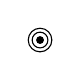
\begin{tikzpicture}[scale=0.5]
    \fill[black] (0,0) circle (0.1);
    \draw (0,0) circle (0.2);
    \draw (0,0) circle (0.3);
  \end{tikzpicture}%
}

\usepackage[clock]{ifsym}


\title{\Huge{Structure de données}\\{IFT2015}\\{\textbf{Introduction}}}
\author{\huge{Franz Girardin}}
\date{\today}
\lstset{inputencoding=utf8/latin1}

            %%%%%%%%%%%%%%%%%  Sect.                          %%%%%%%%%%%%%%%%%%%%%%%%%%%%%%%%%%%%%%%%%%%%%%%%%%%%%%%%%
\usepackage{helvet}
\titleformat{\chapter}[display]
  {\normalfont\bfseries\color{myblue}}
  {\filleft%
    
\begin{tikzpicture}
    \node[
      outer sep=0pt,
      text width=1.5cm,
      minimum height=2cm,
      fill=myblue,
      font=\color{white}\fontsize{40}{50}\selectfont,
      align=center
      ] (num) {\thechapter};
    \node[
      rotate=90,
      anchor=south,
      font=\color{black}\Large\normalfont
      ] at ([xshift=-5pt]num.west) {\textls[180]{\textsc{Section}}};  
    \end{tikzpicture}%
  }
  {5pt}
  {\titlerule[2.0pt]\vskip3pt\titlerule\vskip4pt\large\normalfont}

\titleformat{\section}
  {\normalfont\scshape}{\thesection}{1em}{}



\titleformat{\section}
  {\normalfont\scshape}{\thesection}{1em}{}


% Customizing the spacing for the chapter titles
\titlespacing*{\chapter}{0pt}{0pt}{20pt}

%\usepackage[utopia]{mathdesign}
% Allow hfill in math environment
\newcommand{\specialcell}[1]{\ifmeasuring@#1\else\omit$\displaystyle#1$\ignorespaces\fi}

% Allow you to do the non implication (implication barred)
\newcommand{\notimplies}{%
  \mathrel{{\ooalign{\hidewidth$\not\phantom{=}$\hidewidth\cr$\implies$}}}}



\DeclareRobustCommand{\looongrightarrow}{%
  \DOTSB\relbar\joinrel\relbar\joinrel\relbar\joinrel\rightarrow
}


\title{\Huge{Interface PM}\\{IFT2905}\\{\textbf{Fuille de notes}}}
\author{\huge{Franz Girardin}}
\date{\today}


\begin{document}
\maketitle
\pagebreak
\tableofcontents
\pagebreak
\begin{multicols*}{3}


    \footnotesize
    %\section*{Design of everyday things}

    \chapter{Introduction aux structures de données}
    \section{Caractéristique génériques de $\mathbb{SD}$ }

    \paragraph{Comment décrire une structure de données}
    \begin{itemize}
      \item [$\rhd$ ] \textbf{Linéaire ou \textit{non} linéaire  }  
        \begin{itemize}
          \item [$\blacktriangleright$ ] P. ex. 
            \texttt{graph} vs. \texttt{arrays}    
        \end{itemize}
      \item [$\rhd$ ] Homogène ou non homogène  
        \begin{itemize}
          \item [$\blacktriangleright$ ] Indique si les données sont mê 
            \texttt{type}  
        \end{itemize}
      \item [$\rhd$ ] Statique ou \textit{dynamique}  
        \begin{itemize}
          \item [$\blacktriangleright$ ] P. ex. taille modifiable ou 
            \texttt{fixe}.   
        \end{itemize} 
    \end{itemize}
    
    \begin{note}{}{}
        Plusieurs problèmes ont une complexité telle que les $\mathbb{SD}$ 
        \textbf{base} sont inappropriées, d’où la nécessité 
        des $\mathbb{SD}$ \textbf{abstraites}, plus adéquates.  
    \end{note}

    \paragraph{$\mathbb{SD}$ Abstaites}
    Elles \texttt{généralise} les types de données de base et permettent 
    l'émergence de concept sophistiqués d'\textbf{abstraction}, 
    d'\textbf{encapsulation} et de typage. Elle possèdent 
    \textbf{5 caractéristiques} fondamentales ($\mathbb{TUOPA}$): 
    \begin{itemize}
      \item [$\rhd$ ]  $\mathbb{T}$ype
      \item [$\rhd$ ] $\mathbb{U}$tilise 
      \item [$\rhd$ ] $\mathbb{O}$pérations
      \item [$\rhd$ ] $\mathbb{P}$rocédures
      \item [$\rhd$ ] $\mathbb{A}$xiomes 
    \end{itemize}
    
    \section{Tableau}
    \noindent
    Stocke $\texttt{E}$ dans emplacement de mémoire \textcolor{red}{contigus}.
    \begin{itemize}
      \item [$\rhd$ ] De longueur fixe ou variable
        \begin{itemize}
          \item [$\blacktriangleright$ ] Autrefois : adresse brutes
          \item [$\blacktriangleright$ ] Maintenant : $N$ \texttt{arrays} (indexation)  
          \item [$\blacktriangleright$ ] Maintenant : \texttt{records} (champs)  
        \end{itemize}
    \end{itemize}

    \section{Pile}
    La propriété fondamentale d'une pile est que le seul éléement accessible 
    et celui se trouvant au sommet de la pile. La \textbf{pile}  suit le principe 
    \textbf{LIFO} : \textit{last in, first out}.     



    \section{File}
    La \textbf{file}   suit le principe 
    \textbf{FIFO} : \textit{first in, first out}. Elle possède, entre autres,
    les opération enfiler \textit{enqueue} et défiler \textit{dequeue}.      

    \section{Liste}
    Une file est le résultat de l'\textit{ordonancement} d'un nombre 
    \textcolor{red}{dénombrable} de données où la même valeur 
    peut apparaître plusieurs fois. 

    \begin{itemize}
      \item [$\rhd$ ] \textbf{Implémentation}  
        \begin{itemize}
          \item [$\blacktriangleright$ ] Liste chaînée \texttt{Linked List}  
          \item [$\blacktriangleright$ ] Liste doubleemnt chaînée \texttt{Linked List}  
          \item [$\blacktriangleright$ ] Liste circulaire 

          \item [$\blacktriangleright$ ] Tableau \texttt{array}  
        \end{itemize}
    \end{itemize}


    \begin{note}{}{}
        Une liste chaînée stocke un ensemble d’éléments de 
        façon linéaire. Chaque élément ou nœud d’une liste chaînée 
        contient un \textbf{élément de données} ainsi qu’une 
        \textbf{référence}, ou lien, 
        vers l’élément suivant de la liste.       
    \end{note}


    \section{Arbre} 
    Un arbre stocke un ensemble d’éléments sous une
    forme \textbf{hiérarchique abstraite}. Chaque nœud est relié
    aux autres et peut contenir plusieurs sous-valeurs
    appelées enfants. Il s'agit d'un \texttt{graphe} avec 
    \textbf{3 particularité fondamentales}: 
    \begin{itemize}
      \item [$\rhd$ ] Acyclique
      \item [$\rhd$ ] Connexe
      \item [$\rhd$ ] Possède une seule racine
    \end{itemize}


    \section{File de priorité}
    Possède les mêmes propriété de base qu'un file, sauf que chaque 
    élément a en plus un poids de priorité qui détermine l'ordre 
    global des éléments. 

    \section{Graphe}
    Un graphe stocke un ensemble d’éléments de façon
    non linéaire. Il se compose d’un ensemble fini de
    nœuds, appelés \textbf{sommets}, et de lignes, les arêtes, qui
    relient les sommets entre eux. Les graphes permettent 
    notamment de représenter des systèmes réels, 
    comme des réseaux informatiques.

    \paragraph{Théorème des quatre couleurs}
    Il existe une $4$-coloration de n'importe qu'elle pays 
    qui a été découpé sur une carte. 


    \chapter{Pile}
    \paragraph{Exemples d'applications}
    \begin{itemize}
      \item [$\rhd$ ] Historique de pages visitées
      \item [$\rhd$ ] Annuler une séquence de texte dans un éditeur 
      \item [$\rhd$ ] Chaîne de méthodes appelées d'un fonction complexe
    \end{itemize}

    \paragraph{5 Opération fondamentales}
    \begin{itemize}
      \item [$\rhd$ ] Créer un pile 
      \item [$\rhd$ ] Empiler 
      \item [$\rhd$ ] Dépiler 
      \item [$\rhd$ ] Regarder le sommet 
      \item [$\rhd$ ] Obtenir le nombre d'éléments
    \end{itemize}

    \begin{lstlisting}
elements[0...n-1] <-- tableau // tableau taille n
// top <-- 0 pour assigner 0 à top on fait :

push(E) :
element[top] <-- E
top <-- top + 1 // modifie l'index du sommet 


//  Pour obtenir l'E au sommet, on fait : 

pop() :
retourne element[top] 
top <-- top -1 //decremente la valeur du sommet
x <-- element[top + 1] // enregistre val sommet  
element[top + 1] <-- null
    \end{lstlisting}


    \paragraph{Conventions d'écriture}

    \begin{itemize}
      \item [$\rhd$ ] \textbf{IN}fixé : \texttt{gauche \textcolor{red}{racine} droite}   
        \begin{itemize}
          \item [$\blacktriangleright$ ] 
            $5 \; \textcolor{red}{ - } \;   6 \textcolor{red}{\times} 7
            \leftrightarrow (5 - 6) \times 7 $  
        \end{itemize}
      \item [$\rhd$ ] \textbf{POST}fixé : 
        \texttt{gauche droite \textcolor{red}{racine}}   
        \begin{itemize}
          \item [$\blacktriangleright$ ] 
            $56 \textcolor{red}{ - }   7 \textcolor{red}{\times} 
            \leftrightarrow (56-) \; 7\times$  
        \end{itemize}
      \item [$\rhd$ ] \textbf{PRÉ}fixé : \texttt{\textcolor{red}{racine} gauche droite}  
        \begin{itemize}
          \item [$\blacktriangleright$ ] 
            $\times \textcolor{red}{ - }567 \textcolor{red}{\times} 
            \leftrightarrow \times (-56) \; 7$  
        \end{itemize}
    \end{itemize}


    \paragraph{Avantage de RPN}
    \begin{itemize}
      \item [$\rhd$ ] Aucune ambiguité
      \item [$\rhd$ ] Parenthèses sont superflus 
      \item [$\rhd$ ] Suit la méthodologie calcul des ordinateurs
      \item [$\rhd$ ] Peut être implémentée par une pile
    \end{itemize}


    \paragraph{Méthodtologie RPN pour \texttt{parse} une opératon}

    \begin{enumerate}
      \item Emplier chaque \textbf{opérande} qu'on rencontre dans \texttt{valStack}  
      \item Process quand on rencontre un \textbf{opérateur} : 
        \begin{itemize}
          \item [$\rhd$ ] 
            \texttt{pop} les deux dernières valeurs de la \texttt{valStack}    
          \item [$\rhd$ ] Effectuer l'opération
          \item [$\rhd$ ] \texttt{push} le résultat dans la pile  
        \end{itemize}
    \end{enumerate}

    \end{multicols*}

    \paragraph{Algorithme d'évaluation d'opérations infixée}


    \begin{lstlisting}
       doOp() 
       x = valStack.pop() 
       y = valStack.pop() 
       op = opStack.pop() 
       valStack.push(y op x)

       repeatOps(reOp) 
       tant que (valStack.size > 1) et prec(refOp) < prec(opStack.top()) faire 
          doOp()
        fin tant que 

       EvalExpr() 
       // Entree : flux de jetons representant expression arithmétique
       // Sortie : valeur calculee de l'expression 

       tant que il y a un autre jeton z faire :
          si z est un nombre alors valStack.push(z)
          sinon 
              repeatOps(z)
              opstack.push(z)
        fin tant que

        // Noter que $ est l'opérateur ayant la plus petite precedence 
        repeatOps($) 
        return valStack.top()
    \end{lstlisting}
    \begin{multicols*}{3}


  \chapter{Listes}

  \begin{Definitionx}{}{}
    Un \textbf{type de données abstrait} (ADT) est une abstraction qui définit les
    \textit{opérations} sur les \textit{données} 
    (qui sont physiquement stockées dans une
    structure de données)     
  \end{Definitionx}

  Les ADT spécifient :
  \begin{itemize}
    \item [$\rhd$ ] Données 
    \item [$\rhd$ ] Opération sur les données 
    \item [$\rhd$ ] Cond. d'erreurs associées aux ops. 
  \end{itemize}

  \paragraph{6 Opération fondamentales des listes}
  \begin{itemize}
    \item [$\rhd$ ]
    \item [$\rhd$ ] Créer une liste 
    \item [$\rhd$ ] Ajouter un \texttt{E} à la liste   
    \item [$\rhd$ ] Retirer un \texttt{E} de la liste  
    \item [$\rhd$ ] Vérifier la taille de la liste
    \item [$\rhd$ ] Remplacer un élément par un autre 
    \item [$\rhd$ ] Retrouver un élément 
  \end{itemize}

  \paragraph{Rappel}
  \mbox{}\\
  \noindent Les $k$ premiers termes d'une 
  \textbf{série arithmétique} :  

  \begin{align*}
        & S_n = \sum_{k=0}^{n } k = \frac{n(n+1)}{2} \\ 
        & r = a_n - a_{n-1} \; \forall \; n \geq 2 \\ 
        & a_1 + (n-1)r \;\; \forall \; n \geq 1 
  \end{align*}

  \noindent
  La $k$ premiers termes d'une \textbf{série géométrique} 
  \begin{align*}
        & S_n = \sum_{k=0}^{n } 2k = \frac{1 - 2^{n+1}}{1 - 2} = 2^{n+1} -1 \\ 
        & S_n =  \frac{a(r^{n+1} - 1)}{r - 1} \\ 
        & r = \frac{a_n}{a_{n-1}} \; \forall \; n \geq 2 \\ 
        & a_1 + a_1r^{n-1} \;\; \forall \; n \geq 1 
  \end{align*}


  \paragraph{Opération d'insertion}
  Soit un tableau \texttt{A} de $n$ éléments implémenté 
  par un \texttt{array} indexé de \texttt{0} 
  à \texttt{n - 1}. Et soit $n$ la valeur 
  de l'index pointant vers la prochaine \textbf{case vide}. 
  Les caractéristiques de l'\textcolor{red}{\textbf{opération d'insertion}} 
  sont les suivantes :

  \begin{itemize}
    \item [$\rhd$ ] \texttt{add(i, \textcolor{myb}{x})}  
      \begin{itemize}
        \item [$\blacktriangleright$ ] \textbf{Meilleur temps} : 
          \texttt{i = n} 
        \item [$\rhd$ ] Déplace uniquement \texttt{n}  
        \item [$\rhd$ ] \texttt{n <--- n + 1}     
        \item [$\rhd$ ] \textbf{Temps constant} $O(1)$  
      \end{itemize}
  \end{itemize}


  \begin{itemize}
    \item [$\rhd$ ] \texttt{add(i, \textcolor{myb}{x})}  
      \begin{itemize}
        \item [$\blacktriangleright$ ] \textbf{Pire temps} : 
          \texttt{i = 0} 
        \item [$\rhd$ ] Déplace à droite toute valeur d'index $i \geq 0$     
        \item [$\rhd$ ] 
          \begin{lstlisting}
pour Chaque i<= dex <= n faire :
  A[dex+1] <-- A[dex]             
          \end{lstlisting}
        \item [$\rhd$ ] \textbf{Temps linéaire} $O(n)$  
      \end{itemize}
  \end{itemize}

  En moyenne, le temps pour chaque opération de déplacement est 
  \begin{align*}
      \frac{1}{n}\sum_{i=0}^{n }i = \frac{n(n+1)}{2n} = \frac{n+1}{2} \implies O(n)   
  \end{align*}




  \paragraph{Opération de suppression}
  Soit un tableau \texttt{A} de $n$ éléments implémenté 
  par un \texttt{array} indexé de \texttt{0} 
  à \texttt{n - 1}. Et soit $n$ la valeur 
  de l'index pointant vers la prochaine \textbf{case vide}. 
  Les caractéristiques de l'\textcolor{red}{\textbf{opération de suppresion}} 
  sont les suivantes :

  \begin{itemize}
    \item [$\rhd$ ] \texttt{rem(i, \textcolor{myb}{x})}  
      \begin{itemize}
        \item [$\blacktriangleright$ ] \textbf{Meilleur temps} : 
          \texttt{i = n -1} 
        \item [$\rhd$ ] Déplace uniquement \texttt{null}  
        \item [$\rhd$ ] \texttt{n <--- n - 1}     
        \item [$\rhd$ ] \texttt{A[n] <--- null}     
        \item [$\rhd$ ] \textbf{Temps constant} $O(1)$  
      \end{itemize}
  \end{itemize}


  \begin{itemize}
    \item [$\rhd$ ] \texttt{add(i, \textcolor{myb}{x})}  
      \begin{itemize}
        \item [$\blacktriangleright$ ] \textbf{Pire temps} : 
          \texttt{i = 0} 
        \item [$\rhd$ ] Déplace à gauche toute valeur d'index concernée     
        \item [$\rhd$ ] 
          \begin{lstlisting}
pour Chaque i<= dex <= n - 1 faire :
  A[dex] <-- A[dex + 1]             
          \end{lstlisting}
        \item [$\rhd$ ] \textbf{Temps linéaire} $O(n)$  
      \end{itemize}
  \end{itemize}

  En moyenne, le temps pour chaque opération de déplacement est 
  \begin{align*}
      \frac{1}{n}\sum_{i=0}^{n -1}i = \frac{n(n-1)}{2n} = \frac{n-1}{2} \implies O(n)   
  \end{align*}

  \paragraph{Performance}
  \begin{itemize}
    \item Complexité spaciale de la crétion du tableau : $O(n)$ 
    \item L'idexation d'un \texttt{E} : $O(1)$ 
    \item Opération \textcolor{myb}{\texttt{add}} et 
      \textcolor{myb}{\texttt{remove}} : $O(n)$  
  \end{itemize}

  \paragraph{Agradir un tableau dynamique}
  \begin{itemize}
    \item [$\rhd$ ] Crée un nouveau \texttt{tab} de \texttt{size + 1}    
    \item [$\rhd$ ] Copier les $n$ premiers éléments 
    \item [$\rhd$ ] Ajouter le nouvel élément à l'index $n -1$ 
      (Optionnel)
      du nouveau \texttt{tab}  
    \item [$\rhd$ ] Réaffecter la \texttt{ref} de 
      l'ancient \texttt{tab}   au nouveau \texttt{tab}  
  \end{itemize}

  \begin{lstlisting} 
Algorithme add(x)
// Si aucune E supprime, n aura 
// meme valeur que size
si n = tab1.size() faire :
  Creer nouveau tab de taille voulue 
  pour chaque 0 <= dex n - 1 faire : 
      tab2[i] <-- tab1[i]
  tab1 <-- tab2 
  tab1[n] <-- x
  n <-- n + 1
  \end{lstlisting}


  \section{Liste chaîné}
  La distinction fondamentale entre une liste simple et une liste chaînée 
  est, dans le cas de la liste chaîné, l'existence d'une référence 
  \textbf{indiquant l'emplacement mémoire} du prochain élément de la 
  liste. Et, puisque les \texttt{E} ne sont pas contigus en mémoire, la taille 
  d'une liste chaînée n'a pas unique limite que la quantité 
  de mémoire disponible sur l'ordinateur. 

  \begin{figure}[H]
    \begin{center}
      \includegraphics[width=0.35\textwidth]{ExempleListeChaine.png}
    \end{center}
  \end{figure}


  \begin{Definitionx}{Liste S. chaînée}{}
    Une \textbf{liste simplement chaînée} est une structure 
    de données concrète 
    constituée d'une \textit{séquence de nœuds} à partir
    d'une référence vers 
    le \textbf{noeud de tête}, où chaque nœud 
    contient deux références : 
    vers un \texttt{\textbf{E}}   et vers le \textbf{nœud suivant}. 
    On gardera aussi une référence sur le dernier 
    nœud et un entier 
    pour le nombre d’éléments dans la liste.     
  \end{Definitionx}

  \begin{figure}[H]
    \begin{center}
      \includegraphics[width=0.33\textwidth]{ListeSChainee.png}
    \end{center}
  \end{figure}



  \begin{lstlisting}
   initialisation(varElement, varNext)
   element <-- varElement // Assigne E
   next <-- varNext  // specifie prochain noeud


   Class LinkList(List) 
   initialisation()
   head <-- null 
   next <-- null 
   size <-- 0

   fonction len() 
      retourner size 

  fonction str() 
    Si isEmpty() 
      retourner "[] (size = 0)"
    Si non : 
    PP <- "["
    curr <- head 
    tant que curr != null faire 
      // (concat)
      PP <- PP + curr.next + " " 
      curr <- curr.next

    Fin tant que 

    PP <- PP + "]" 
    PP <- PP + "(size = " + size +")"

  fonction isEmpty() 
      retourner size = 0
  \end{lstlisting}

  \section{Liste doublement chaînée}
  \begin{Definitionx}{Liste D. chaînée}{}
    Une \textbf{liste doublement chaînée} est une structure de 
    données constituée d'une \textit{séquence de nœuds} à partir 
    de références vers les nœuds de tête et de queue, 
    où chaque nœud contient \textbf{trois références} : 
    vers un \texttt{\textbf{E}}  , 
    vers le \textbf{nœud suivant} et vers le \textbf{nœud précédent}.
    On gardera aussi un entier pour le nombre d’éléments 
    dans la liste.     
  \end{Definitionx}

  \begin{lstlisting}
Class DoublyLinkedNode() 

// Methode generale d'initialisation
initialisation(varE, varPrev, varNext) 
  element <-- varE 
  prev <-- varPrev 
  next <-- varNext 


// initialisation pour 
// engendrer la fonction str()


initialisation()
  head <-- DoublyLinkedNote(null, null, null)
  tail <-- DoublyLinkedNode(null, null, null) 
  head.next <-- tail
  tail.prev <-- head 
  size <-- 0 

fonction len() 
  retourner size 

fonction str() 
  Si isEmpty() 
    retourner 
    "[] (size = 0)"
  Sinon :
    PP <-- "[" 
    curr <-- head.next

    tant que curr.next != tail faire :
      PP <-- PP + curr.element + "" 
      curr <-- curr.next 
    Fin tant que 

    PP <-- PP + "]" + 
    "size = (" + size + ")"
  Fin si 

fonction isEmpty() 
  retourner size = 0

  \end{lstlisting}

  \chapter{Liste généralisée}
  \begin{Definitionx}{Liste G.}{}
      Liste dans laquelle les éléments 
      peuvent être des sous-listes 
      Si un \texttt{E} de la liste 
      \textbf{n'est pas} une sous-liste, il est dit 
      \textcolor{red}{atomique}. Les liste 
      généralisées peuvent être représentées 
      par des représentations 
      séquentielles ou chaînées. 
  \end{Definitionx}

  \paragraph{Liste généralisée 1}
  \begin{lstlisting}
(a_1, a_2, 
  (b_1, 
    (c_1, c_2), 
  b_3), 
a_4, 
  (d_1, d_2) 
a_6) 
  \end{lstlisting}

  \begin{note}{}{}
      On utilise \textbf{0} pour représenter un 
      atome et \textbf{1} pour représenter une 
      sous-liste (Parfois T/F)
  \end{note}

  \paragraph{Liste généralisée 2}
  \begin{figure}[H]
    \begin{center}
      \includegraphics[width=0.33\textwidth]{ListeGen2.png}
    \end{center}
  \end{figure}

  \paragraph{Liste généralisée 3}

  \begin{figure}[H]
    \begin{center}
      \includegraphics[width=0.33\textwidth]{Listegen.png}
    \end{center}
  \end{figure}


  \chapter{File}
  Pour l'implémentation, on utilise un tableau circulaire de 
  \textcolor{red}{taille $N$}, ainsi que 
  \textit{deux variables} qui gardent trace de 
  l'\textbf{avant} et l'\textbf{arrière} : 
  \textcolor{red}{$f$} et \textcolor{red}{$r$}.       
  \begin{itemize}
    \item [$\rhd$ ] \textcolor{red}{$f$} 
      index directement sur la valeur  
    \item [$\rhd$ ] \textcolor{red}{$r$} 
      index 1ere case vide après valeur. 
  \end{itemize}


  \begin{figure}[H]
    \begin{center}
      \includegraphics[width=0.33\textwidth]{FileSurTableau.png}
    \end{center}
  \end{figure}

  \begin{lstlisting}
// Algorithme size() 
retourne (r - f + N) mod N 

// Algorithme isEmpty() 
retourn (f = r)


// Algorithme Enqueue(x) 
Si size() = N - 1 faire : 
  retourne Erreur 
Sinon : 
  Q[r] <-- x 
  r <-- (r+1) mod N


// Algorithme Dequeue()
Si Q iseEmpty() faire : 
  retourne erreur 
Sinon :
  x <-- Q[f] 
  f <-- (f + 1) mod N 
  retourne x
  \end{lstlisting}


  \paragraph{Variante}
  \begin{itemize}
    \item [$\rhd$ ] \textcolor{red}{$f$} 
      index directement sur la valeur  
    \item [$\rhd$ ] \textcolor{red}{$r$} 
      
      index \textcolor{red}{directement sur case fin}. 
  \end{itemize}

\begin{lstlisting}
 // Algorithme size() 
retourne ((r - f + N) mod N) + 1

// Algorithme isEmpty() 
retourne (f = (r + 1) mod N)

// Algorithme Enqueue(x) 
Si ((r + 1) mod N) = f alors 
  retourne Erreur // La file est pleine
Sinon : 
  Q[r] <-- x 
  r <-- (r + 1) mod N

// Algorithme Dequeue()
Si isEmpty() alors 
  retourne erreur 
Sinon :
  x <-- Q[f] 
  f <-- (f + 1) mod N 
  retourne x
\end{lstlisting}
  
  
  
  
  






    














    \end{multicols*}


\end{document}

